\subsubsection{subfunction-oeSendPoliceReport}

\label{RE-use-case-oeSendPoliceReport}


To send a report to Police Headquarters about a crisis near to location		  


\begin{usecase}
  \addheading{Use-Case Description}
  \addsingletwocolumnrow{Name}{oeSendPoliceReport}
  \addsingletwocolumnrow{Scope}{system}
  \addsingletwocolumnrow{Level}{subfunction}
  
\addrowheading{Parameters}
\addnumberedsinglerow{AdtReport: dtReport}{}

\addrowheading{Primary actor(s)}
\addnumberedsinglerow{}{\msrcode{actCoordinator[active]}}


\addrowheading{Secondary actor(s)}
\addnumberedsinglerow{}{\msrcode{actPoliceHeadquarter[passive, multiple]}}

\addrowheading{Goal(s) description}
\addsinglerow{To send a report to Police Headquarters about a crisis near to location}

\addrowheading{Protocol condition(s)}
\addnumberedsinglerow{}{
there is a coordinator and a crisis created in the system 
}

\addrowheading{Pre-condition(s)}
\addnumberedsinglerow{}{
the crisis associated in the report must be handled by the coordinator who want to send it
}

\addrowheading{Main post-condition(s)}
\addnumberedsinglerow{}{
send report in SMS message to police headquarters nearest to crisis location
}

\addrowheading{Additional Information}
\addsinglerow{
none
}

\end{usecase} 

Figure \ref{fig:lu.uni.lassy.excalibur.examples.icrash-RE-UCD-uc-oeSendPoliceReport}
 send a crisis report to the police headquarters near to the crisis

\begin{figure}[htbp]
\begin{center}

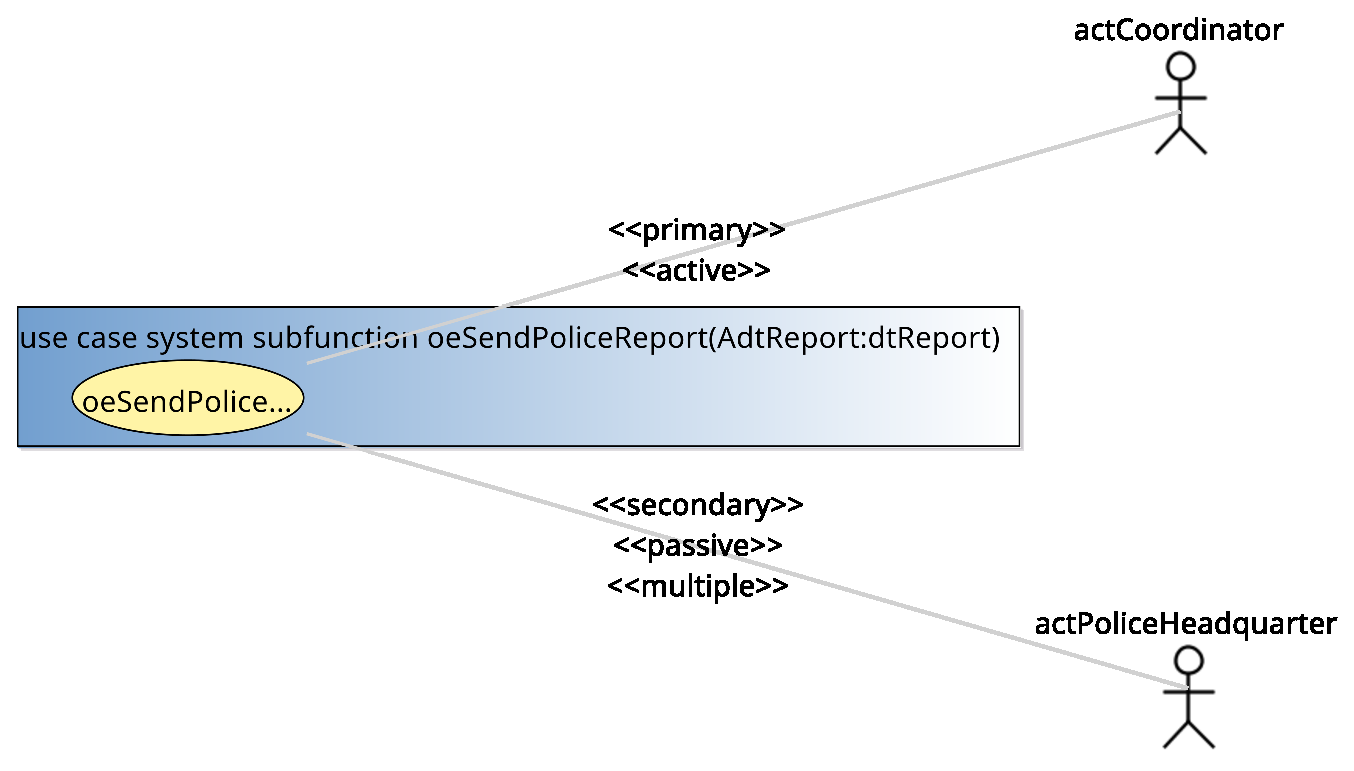
\includegraphics[
angle=0
]{./images-report-gen/usecase-model/subfunction/uc-oeSendPoliceReport.eps}
\end{center}
\caption[lu.uni.lassy.excalibur.examples.icrash Use Case Diagram: uc-oeSendPoliceReport]{}
\label{fig:lu.uni.lassy.excalibur.examples.icrash-RE-UCD-uc-oeSendPoliceReport}
\end{figure}
\vspace{0.5cm}
